\documentclass{beamer}
\usepackage{relsize}
\usepackage{color}

\usepackage{listings}
\usetheme{CambridgeUS}
%\usepackage{beamerthemesplit} % new
\usepackage{enumitem}
\usepackage{amsmath}                    % See geometry.pdf to learn the layout options.
\usepackage{amsthm}                   % See geometry.pdf to learn the layout options. There
\usepackage{amssymb}                    % See geometry.pdf to learn the layout options.
\usepackage[utf8]{inputenc}
\usepackage{graphicx}
\usepackage[english,bulgarian]{babel}

\usepackage{caption}
\usepackage{tikz}
\usepackage{forest}

\usetikzlibrary{shapes,arrows,positioning,calc,positioning,fit,chains}

\usetheme{CambridgeUS}
\usecolortheme{crane}

\lstset{language=C++,
                basicstyle=\ttfamily,
                keywordstyle=\color{blue}\ttfamily,
                stringstyle=\color{red}\ttfamily,
                commentstyle=\color{green}\ttfamily,
                morecomment=[l][\color{magenta}]{\#}
}

\tikzset{
block/.style = {draw, fill=white, rectangle,align = center},
entry/.style = {draw, fill=black, circle, radius=3em},
condition/.style = {draw, fill=white, diamond, align = center,node distance=3cm},
fork/.style = {draw, fill=black, circle,inner sep=1pt},
lnode/.style={rectangle split, rectangle split parts=3,draw, rectangle split horizontal},
treenode/.style = {align=center, inner sep=0pt, text centered, circle, font=\sffamily\bfseries, draw=black, fill=white, text width=1.5em},
flexnode/.style = {align=center, text centered, ellipse, font=\sffamily\bfseries, draw=black, fill=white},
token/.style={rectangle split, rectangle split parts=2,draw, rectangle split horizontal=false}
}


\newtheorem{mydef}{Дефиниция}[section]
\newtheorem{lem}{Лема}[section]
\newtheorem{thm}{Твърдение}[section]

\DeclareMathOperator{\restrict}{\upharpoonright}

\setitemize{label=\usebeamerfont*{itemize item}%
  \usebeamercolor[fg]{itemize item}
  \usebeamertemplate{itemize item}}

\setbeamercovered{transparent}

\captionsetup{font=tiny} 

\begin{document}
\title[Стекове и опашки]{Стекове и опашки. Реализация и приложения}
\frame{\titlepage}

\section{Какво е стекова организация?}
\subsection{}


\begin{frame}[fragile]
\frametitle{Train shunting}

\begin{tikzpicture}[remember picture,overlay]
  \node[xshift=0mm,yshift=-15mm,anchor=north] at (current page.north){%
  
\includegraphics[width=150mm]{images/trains 1}};
\end{tikzpicture}

\end{frame}


\begin{frame}[fragile]
  \frametitle{Train shunting}
  
  \begin{tikzpicture}[remember picture,overlay]
    \node[xshift=0mm,yshift=-15mm,anchor=north] at (current page.north){%
    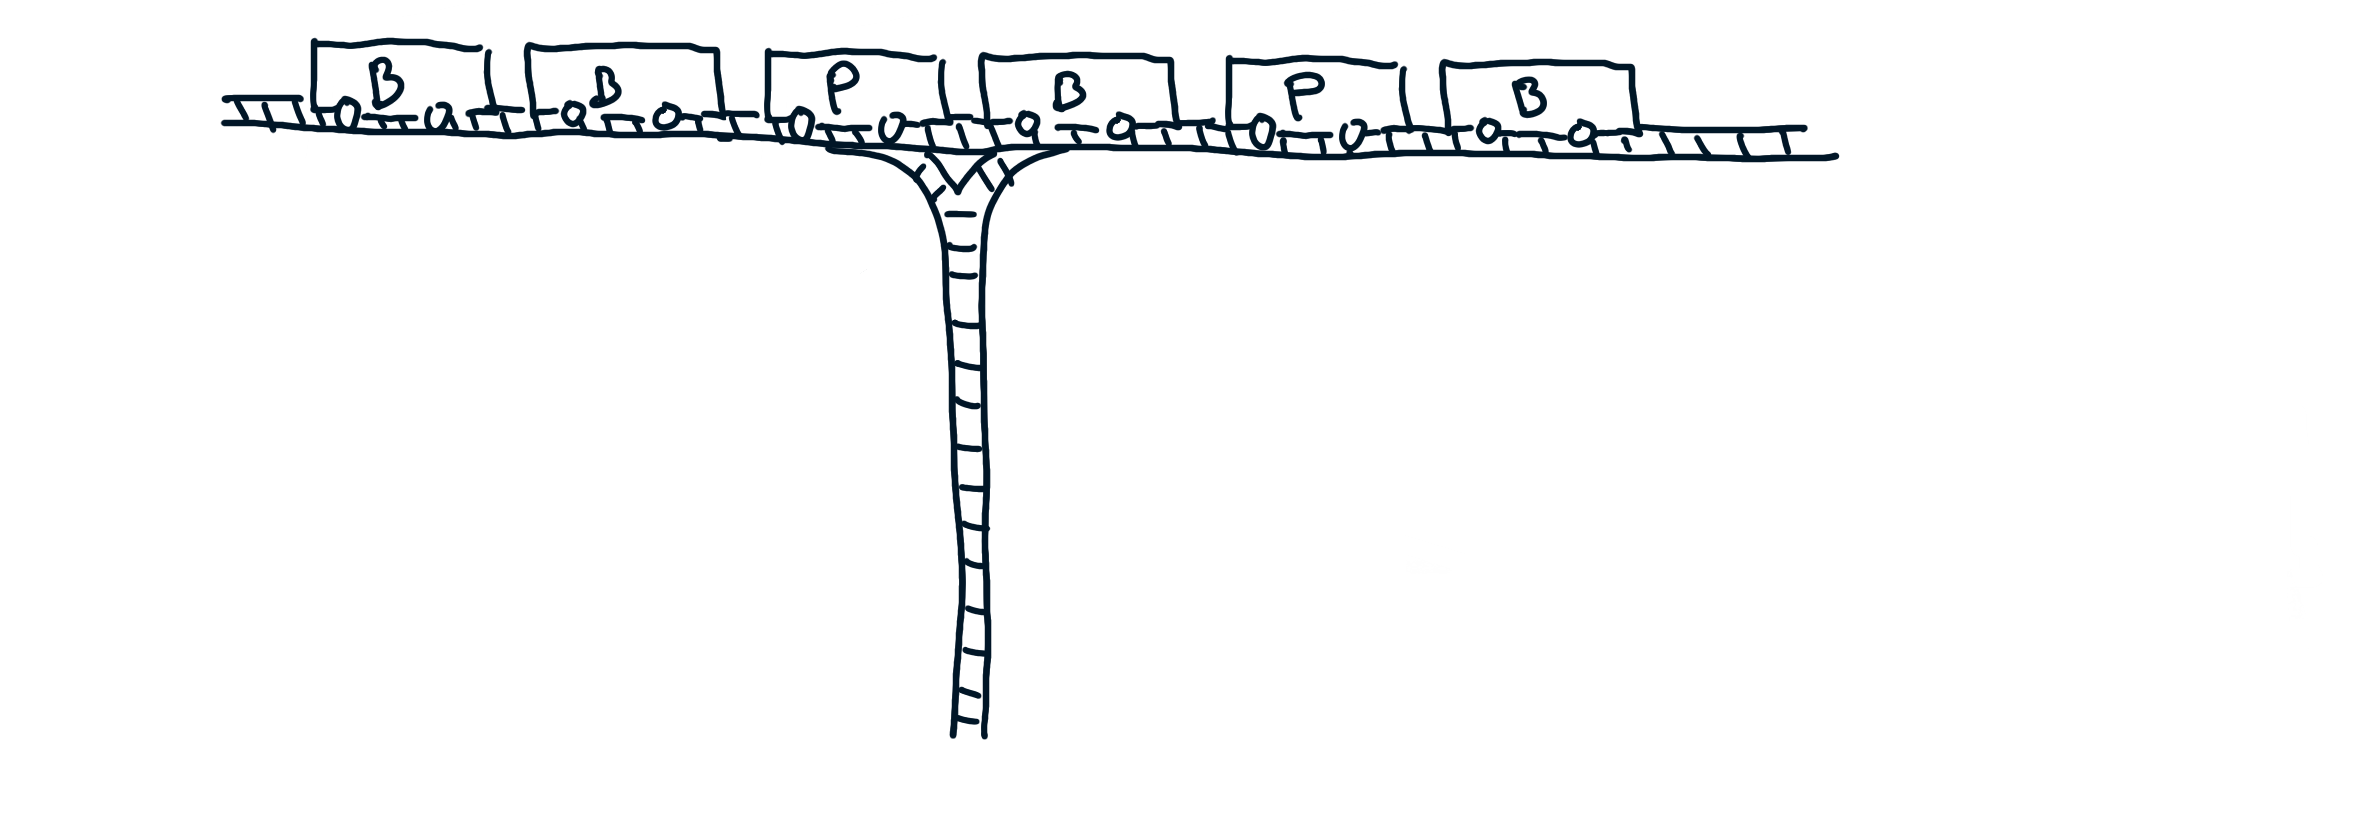
\includegraphics[width=150mm]{images/trains 2}};
  \end{tikzpicture}
  
\end{frame}

\begin{frame}[fragile]
  \frametitle{Train shunting}
  
  \begin{tikzpicture}[remember picture,overlay]
    \node[xshift=0mm,yshift=-15mm,anchor=north] at (current page.north){%
    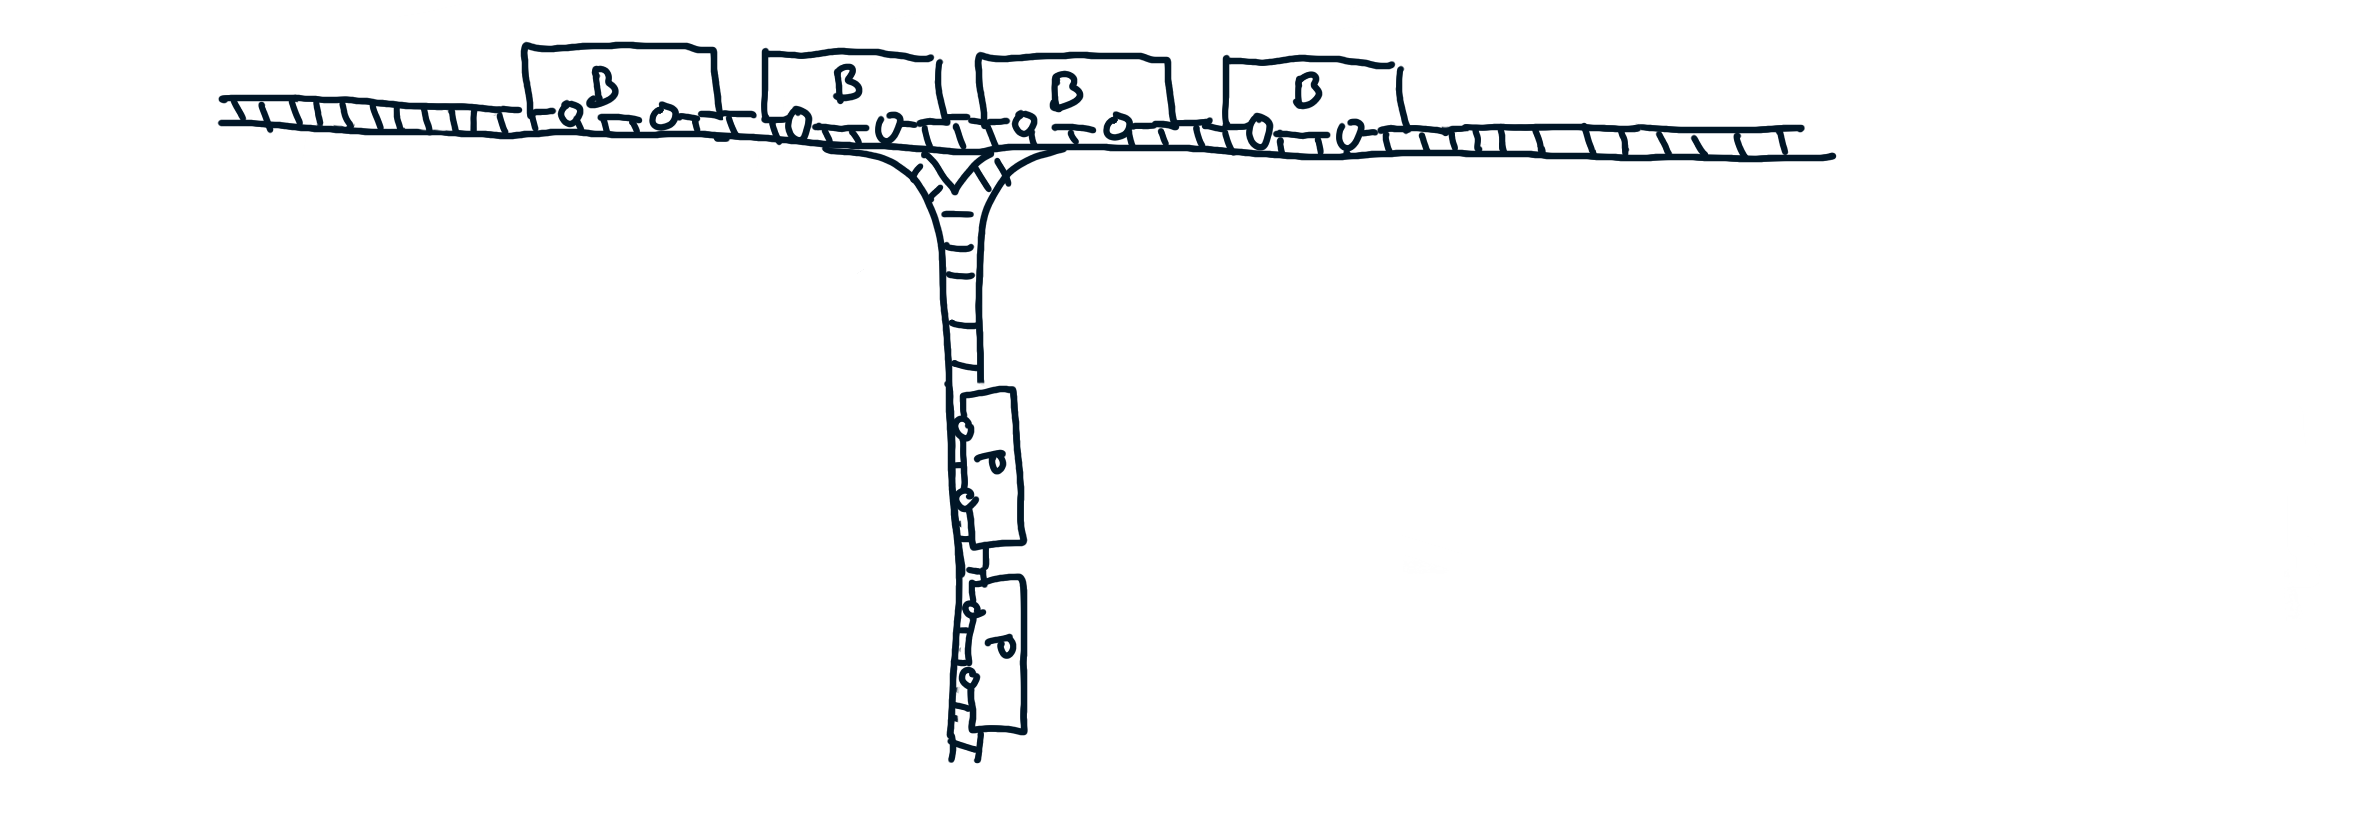
\includegraphics[width=150mm]{images/tranis 3}};
  \end{tikzpicture}
  
\end{frame}
 

\begin{frame}
  \centerline{Обратен полски запис}
  \centerline{Reversed Polish Notation (RPN)}
  \end{frame}
  
  \begin{frame}[fragile]
  \frametitle{Обратен полски запис}

  \begin{tikzpicture}[remember picture,overlay]
    \node[xshift=0mm,yshift=-15mm,anchor=north east] at (current page.north east){%
    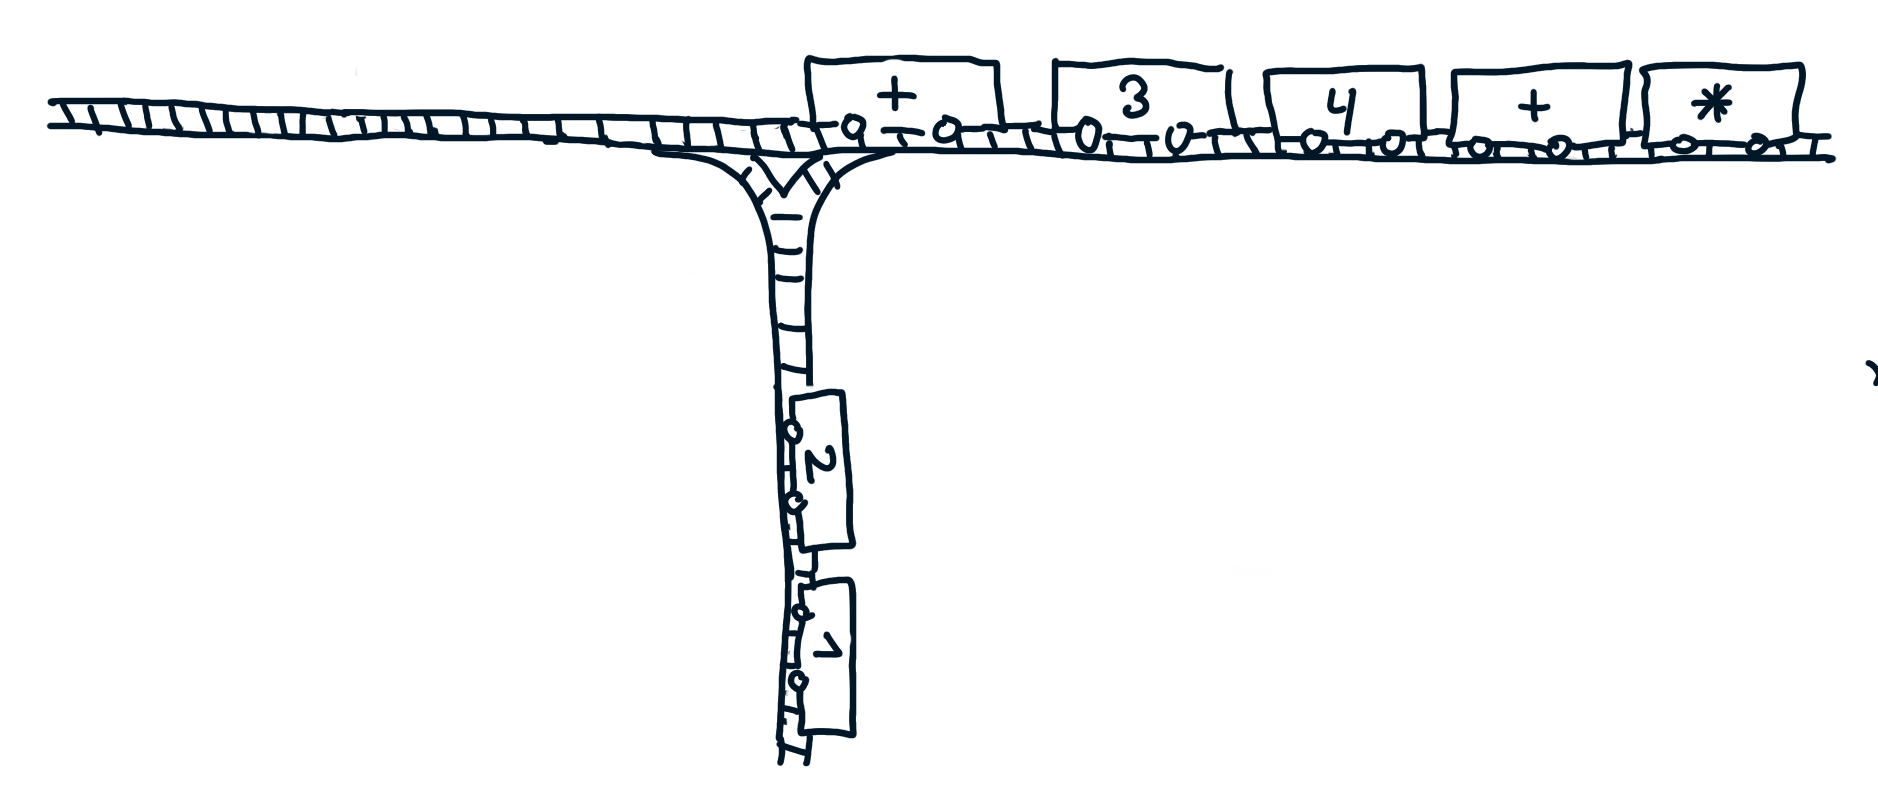
\includegraphics[width=90mm]{images/rpn 1}};
  \end{tikzpicture}
  

  \relscale{0.8}
  \begin{verbatim}
  (1 + 2) * (3 + 4)
  1 2 + 3 4 + *  
  \end{verbatim}
  
  \begin{itemize}
    \item Оценка със стек
  \end{itemize}
  
  \end{frame}
  
  

\begin{frame}
\centerline{Shunting Yard Алгоритъм}
\end{frame}


\begin{frame}[fragile]
  \frametitle{Shunting Yard}
  \begin{figure}
    \centering
    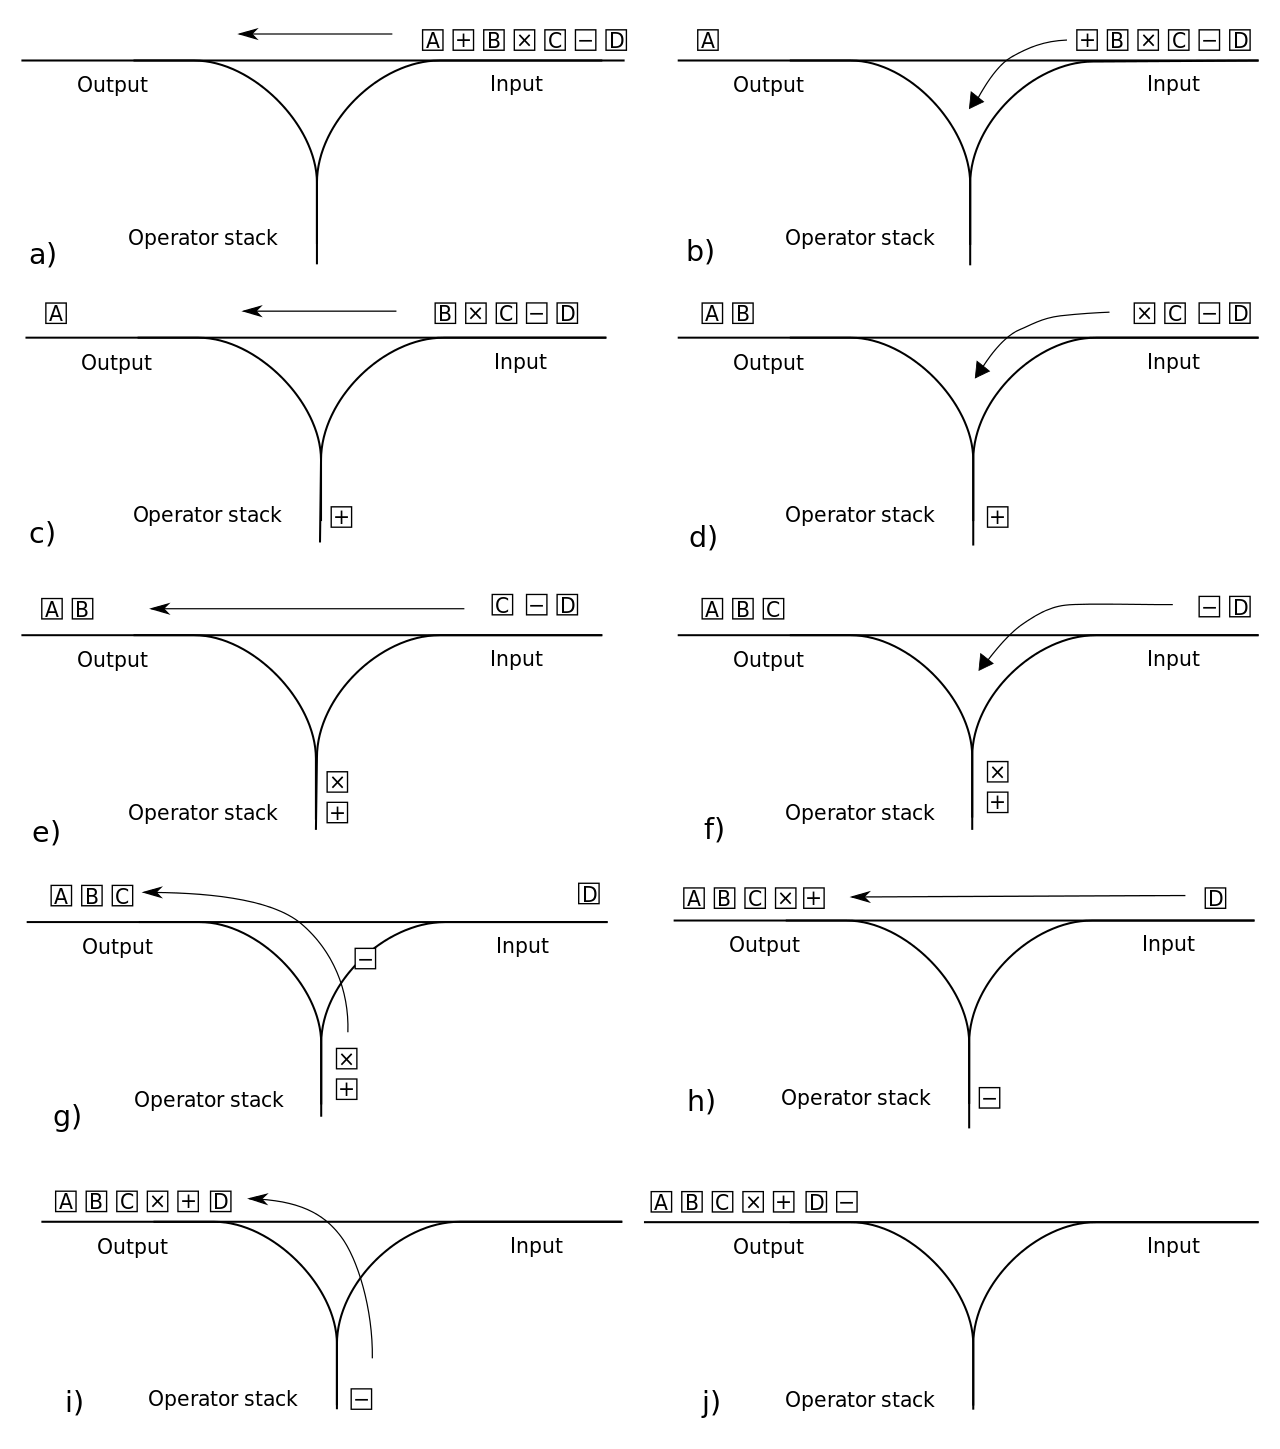
\includegraphics[width=6cm]{images/shunting_yard}
    \caption{Алгоритъм Shunting Yard. Източник: \href{https://en.wikipedia.org/wiki/Shunting-yard_algorithm}{Wikipedia}}
    \label{fig:syard}
    \end{figure}  
\end{frame}
  

\begin{frame}[fragile]
  \frametitle{Shunting Yard}
  \begin{itemize}
    \item Число: директно отива в изхода
    \item Оператор: изважда от върха на стека всички оператори с по-голям или равен приоритет
    \item Отваряща скоба: застава на върха на стека
    \item Затваряща скоба: изважда от стека всичко до отварящата скоба, като маха и нея
  \end{itemize}
\end{frame}

\begin{frame}[fragile]
  \frametitle{Стекова организация}

  \begin{tikzpicture}[remember picture,overlay]
    \node[xshift=0mm,yshift=-15mm,anchor=north] at (current page.north){%
    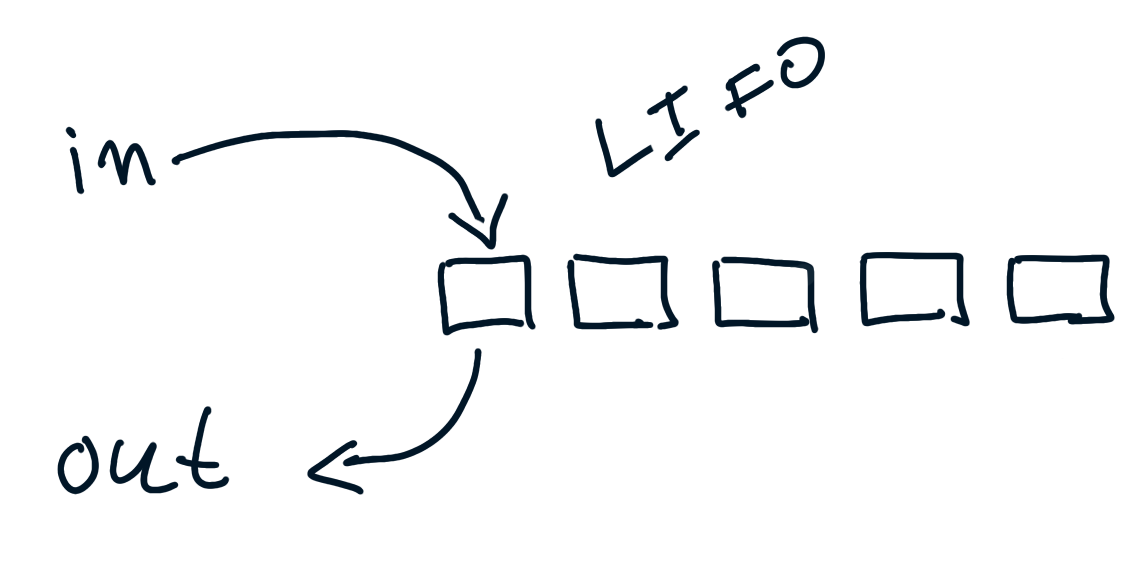
\includegraphics[width=90mm]{images/lifo}};
  \end{tikzpicture}

\end{frame}  


\begin{frame}
  \centerline{Опашка}
\end{frame}
  
\begin{frame}[fragile]
  \frametitle{Опашка}

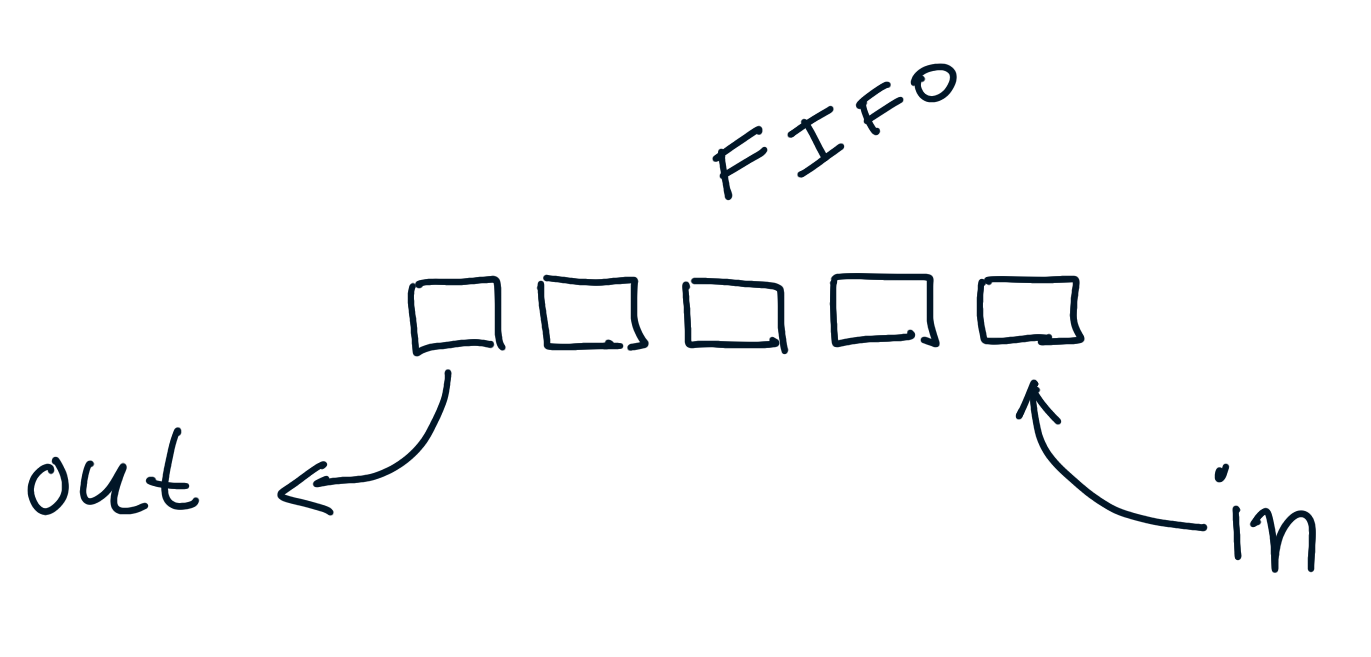
\includegraphics[width=90mm]{images/fifo};

\begin{lstlisting}[basicstyle=\small,language=Haskell]
push q x = q ++ [x]
top q = head q
pop q = tail q
\end{lstlisting}
  
\begin{itemize}
  \item Всяко вмъкване на елемент води до дублиране на целия списък
\end{itemize}

\end{frame} 

\begin{frame}
  \centerline{Обхождане в широчина}
\end{frame}

\begin{frame}[fragile]
  \frametitle{Breadth-first search (BFS)}

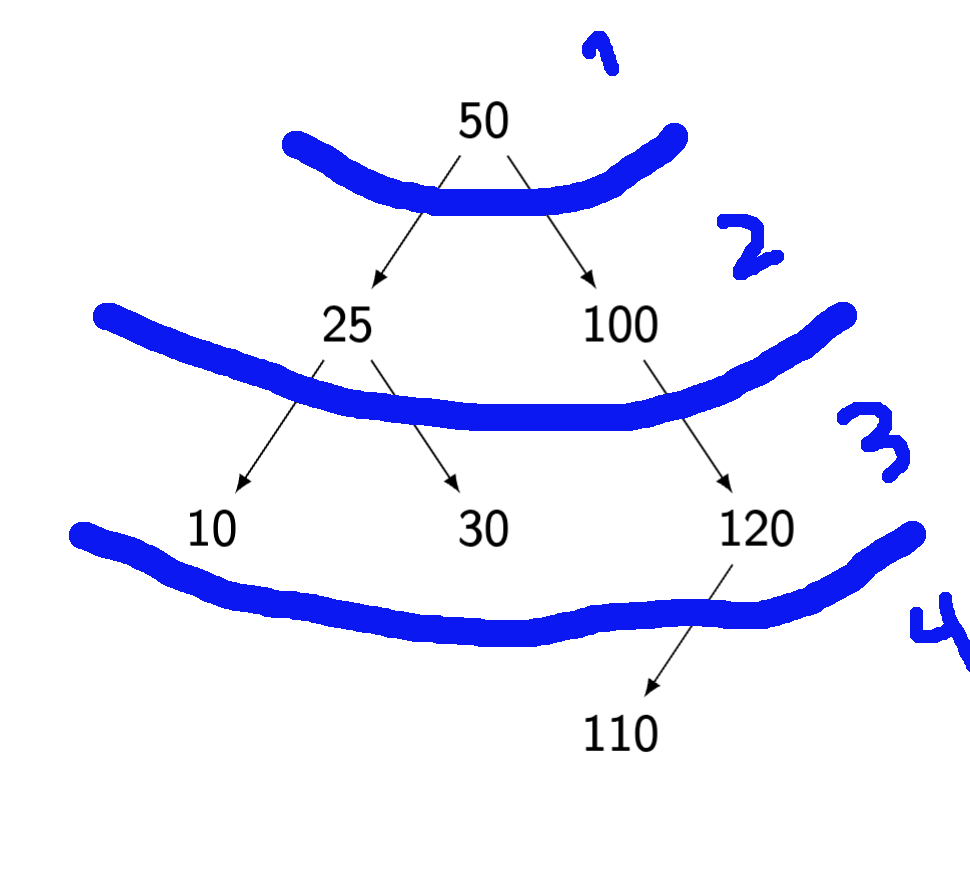
\includegraphics[width=60mm]{images/bfs};

\end{frame} 


\begin{frame}[fragile]
  \frametitle{Breadth-first search (BFS)}

\begin{tikzpicture}[remember picture,overlay]
  \node[xshift=0mm,yshift=-35mm,anchor=north west] at (current page.north west){%
  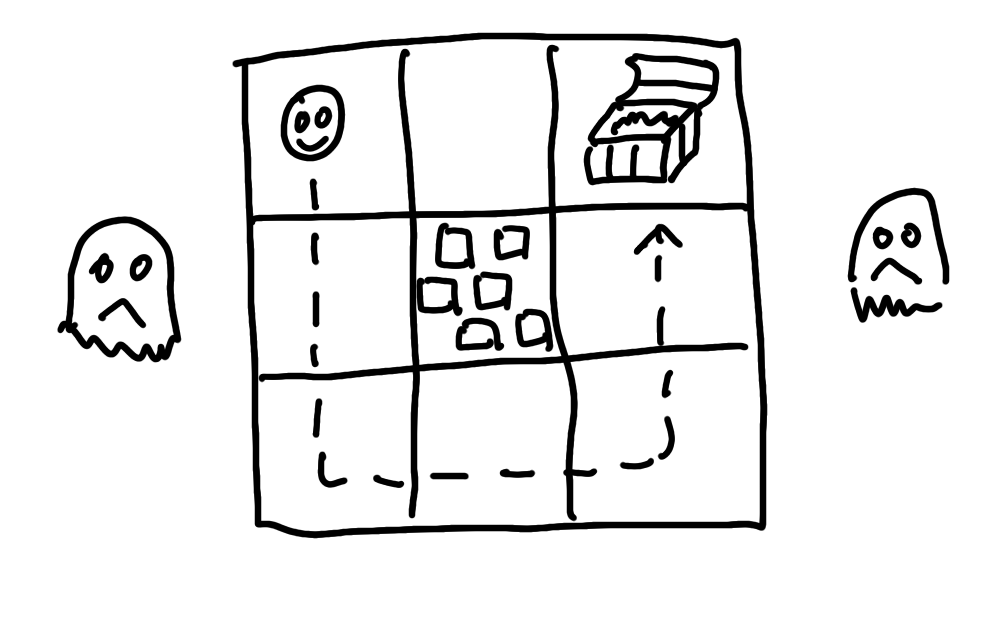
\includegraphics[width=60mm]{images/maze}};
  \node[xshift=0mm,yshift=-35mm,anchor=north east] at (current page.north east){%
  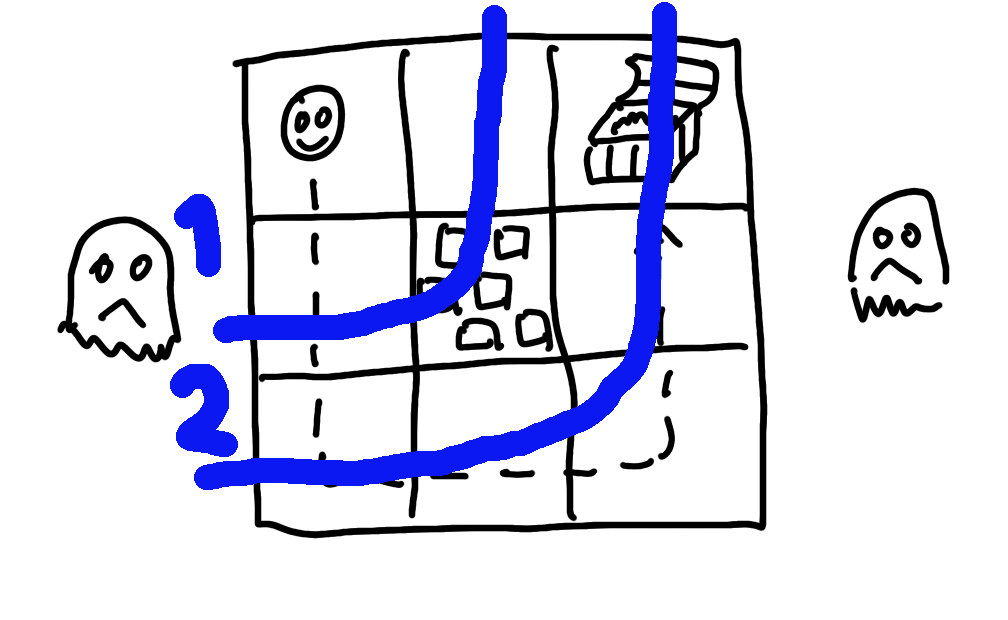
\includegraphics[width=60mm]{images/maze2}};
\end{tikzpicture}

\end{frame} 

\begin{frame}[fragile]
  \frametitle{Реализация на опашка чрез стекове}

  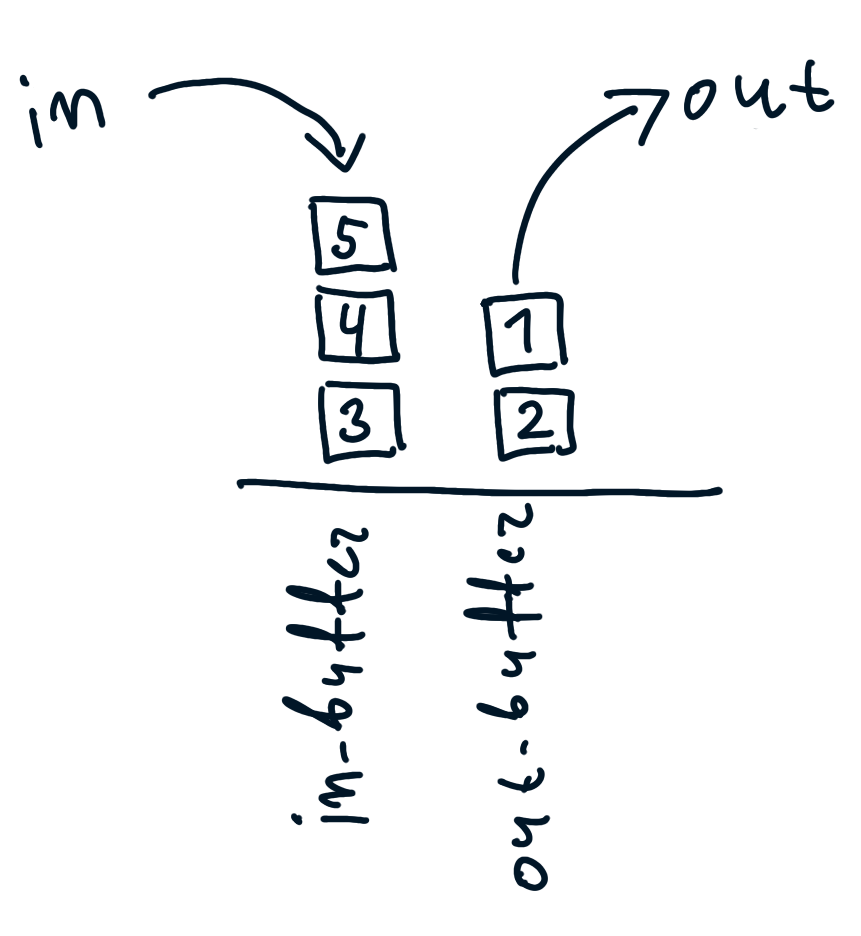
\includegraphics[width=60mm]{images/qstack};

\end{frame} 


\begin{frame}
  \centerline{Благодаря за вниманието!}
\end{frame}


\end{document}


\begin{columns}[t]
  \begin{column}{0.3\textwidth}

  \end{column}
  \begin{column}{0.7\textwidth}

  \end{column}
\end{columns}


\begin{lstlisting}[basicstyle=\small,language=Haskell]
\end{lstlisting}
